\pdfoutput=1
\documentclass[11pt]{amsart}
\usepackage[margin=1.2in]{geometry}
\usepackage{amsmath,amssymb,amsthm,graphicx}
\usepackage[hidelinks]{hyperref}
\raggedbottom
\usepackage{microtype}
\linespread{1.15}
\setlength{\parskip}{4pt plus 1pt}
\AtBeginDocument{%
  \setlength{\abovedisplayskip}{12pt plus 2pt}\setlength{\belowdisplayskip}{12pt plus 2pt}%
  \setlength{\abovedisplayshortskip}{8pt plus 2pt}\setlength{\belowdisplayshortskip}{8pt plus 2pt}}
\newcommand{\step}[1]{\par\medskip\noindent\emph{#1}\ }
\newtheorem{theorem}{Theorem}
\newtheorem{lemma}[theorem]{Lemma}
\theoremstyle{remark}
\newtheorem{remark}[theorem]{Remark}
\newcommand{\E}{\mathbb{E}}
\newcommand{\Var}{\operatorname{Var}}
\newcommand{\Cov}{\operatorname{Cov}}
\newcommand{\C}{\mathbb{C}}
\newcommand{\R}{\mathbb{R}}

\title[Hairpins and basepairs are jointly normal]{Hairpins and basepairs in RNA secondary structures are asymptotically jointly normal: proof of a conjecture of Bu, Kauers and Zeilberger}
\author{Brian Sheppard}
\thanks{The mathematics in this note was produced by Claude (Anthropic) at the author's direction; see ``How this note was made'' in Section~1. arXiv policy does not permit listing an AI system
as an author, so the author line names the person responsible for the submission.}
\email{bshepp@gmail.com}
\date{October 2026. Not a conventional paper: see ``How this note was made'' in Section 1.}

\begin{document}
\begin{abstract}
Bu, Kauers and Zeilberger conjectured that the numbers of hairpins and of basepairs in a uniformly random
RNA secondary structure on $n$ vertices are, after centring and scaling, asymptotically bivariate normal with
correlation $\tfrac12\sqrt{5\sqrt5-11}=0.21233\ldots$. This note gives a rigorous proof. The method is the standard one
(a square-root singularity that moves analytically with the marking variables, hence a quasi-power expansion of
the moment generating function); a bivariate normal law for these two parameters was derived along these lines, at
a heuristic level and for a family of models containing this one, by Cuesta and Manrubia in 2017, and the statement
also follows from a general theorem of Drmota once its hypotheses are checked. What is done here is to check them:
a short self-contained proof with a uniform coefficient estimate, the limiting mean vector and covariance matrix in
closed form, and a verification of every algebraic identity used in the proof, both in Mathematica and in the Lean~4 proof
assistant. The mathematics was produced by an AI system; the human role was direction, verification protocol and
transparency, and is described in Section~1.
\end{abstract}
\maketitle

\section{Statement}
A \emph{secondary structure} on $[n]=\{1,\dots,n\}$ is a set of pairwise disjoint pairs $\{i,j\}$
(\emph{basepairs}) with $j-i\ge 2$ and no crossings (no $i<k<j<l$ with $\{i,j\},\{k,l\}$ both present).
A basepair $\{i,j\}$ is a \emph{hairpin} if none of $i+1,\dots,j-1$ is paired. For a uniformly random secondary
structure on $[n]$ let $X_n$ be its number of hairpins and $Z_n$ its number of basepairs.
In \cite{BKZ} the following is conjectured, with a pledge of \$100 to the OEIS Foundation for a proof.

\begin{theorem}\label{main}
As $n\to\infty$,
\[
\left(\frac{X_n-\E X_n}{\sqrt{\Var X_n}},\ \frac{Z_n-\E Z_n}{\sqrt{\Var Z_n}}\right)\ \xrightarrow{\ d\ }\
\mathcal N\!\left(0,\begin{pmatrix}1&c\\ c&1\end{pmatrix}\right),\qquad c=\frac{\sqrt{5\sqrt5-11}}{2}.
\]
Moreover, with
\[
\mu=\Bigl(1-\tfrac{2}{\sqrt5},\ \tfrac{5-\sqrt5}{10}\Bigr),\qquad
H=\begin{pmatrix} 2-\frac{22}{5\sqrt5} & \frac{25-11\sqrt5}{50}\\[2pt] \frac{25-11\sqrt5}{50} & \frac{1}{10\sqrt5}\end{pmatrix},
\qquad \det H=\tfrac{13\sqrt5-29}{50}>0,
\]
we have $(\E X_n,\E Z_n)=n\mu+O(1)$ and the covariance matrix of $(X_n,Z_n)$ is $nH+O(1)$.
\end{theorem}

\begin{remark}
The density displayed in \cite{BKZ}, $\frac{\sqrt{1-c^2}}{2\pi}e^{-x^2/2-y^2/2+cxy}$, is that of the centered
normal law with covariance matrix $(1-c^2)^{-1}\bigl(\begin{smallmatrix}1&c\\c&1\end{smallmatrix}\bigr)$, whose
marginals have variance $1/(1-c^2)=1.0472\ldots$; this cannot be the limit of coordinates standardized to
variance one. The conjecture is read here as its text and abstract state it: bivariate normal with unit variances and
correlation $c$, whose density is
$\frac{1}{2\pi\sqrt{1-c^2}}\exp\bigl(-\frac{x^2-2cxy+y^2}{2(1-c^2)}\bigr)$.
\end{remark}

\subsection*{Related work and what is new}
Nothing in the method is new. For a quadratic generating function with a simple dominant branch point, Gaussian
limit laws follow from the ``algebraic singularity schema'' \cite[Thm.~IX.12]{FS} (one parameter) and its
multivariate versions \cite{BR,GR}, \cite[Thm.~2.25]{D}, \cite{HK}; see also \cite[\S IX.12 (multivariate limit laws)]{FS}.
For RNA secondary structures specifically:
\begin{itemize}
\item Jin and Reidys \cite{JR} proved central and local limit theorems for the number of basepairs alone, with the
same mean and variance constants $\tfrac{5-\sqrt5}{10}$ and $\tfrac1{10\sqrt5}$ (numerically, $0.27639$ and $0.04472$).
\item Cuesta and Manrubia \cite[\S3.3]{CM} treat the pair (basepairs, hairpins) in the family of models with stems
of length $\ge s$ and hairpin loops of size $\ge m$. They obtain the expansion \eqref{qp} below from Darboux's
theorem and read off a bivariate normal law, with numerical constants for $(s,m)=(2,3)$. Their argument is at the
level of rigour customary in physics: the coefficient asymptotics are applied for each fixed value of the marking
variables, without the uniformity that the continuity theorem requires, and non-degeneracy is not discussed. The
model of \cite{BKZ} is the case $s=m=1$: their discriminant $\Delta(z,w,u)$ satisfies $(1-z)^2\Delta=R$ identically,
with $R$ as in Lemma~\ref{gf}. As a check on both computations, the script \texttt{checks/cuesta\_manrubia.wls} reproduces all the
constants they publish for $(2,3)$.
\item Poznanovi\'c and Heitsch \cite{PH} prove univariate Gaussian laws for motif counts in a stochastic context-free
grammar model of RNA folding, also via \cite[Thm.~IX.12]{FS}.
\end{itemize}
What this note adds is a complete proof for the model and normalization of \cite{BKZ}: the hypotheses (a unique simple
dominant root, non-vanishing of the square-root coefficient, non-singularity of the Hessian) are verified exactly,
the uniform estimate is proved directly (Lemma~\ref{coef}) so that the argument can be read without the general
theory, and the constants are obtained in closed form in $\mathbb Q(\sqrt5)$. A reader who prefers to quote a theorem
can stop after Section~3: the representation \eqref{AB}, with $\rho$, $A$, $B$ analytic for $|X|<0.51$ and
$B(\rho)\neq0$, supplies the hypotheses of \cite[Thm.~2.25]{D} with exponent $\tfrac12$, and the limit is
non-degenerate because $\det H\neq0$ (Section~5). Alternatively, Lemma~\ref{coef} is precisely the hypothesis of
the multivariate central limit theorems of Bender and Richmond \cite[Thm.~1]{BR} and Gao and Richmond
\cite[Thm.~2]{GR}, whose proofs Section~5 reproduces in this special case; \cite[Thm.~4]{GR} then gives a local
limit theorem as well.

\subsection*{How this note was made}
This is not a conventional paper and I (Brian Sheppard) am not its mathematician. I am a software engineer with a course
in mathematical thinking and one undergraduate paper, on topological robot motion planning \cite{JSZ}. In the course of this work I learned what a secondary structure and a
hairpin are and how the argument is built; I can follow its logic in outline and I know what questions to ask of
it. I could not have produced it and I cannot certify it.

Everything mathematical here was produced by Anthropic's Claude (Claude Fable 5.1, run as the Claude Code agent):
the proof strategy, the proof, the text of this note outside this section and the first draft of this section,
the Mathematica and Lean code, and the literature search. My part was the
pipeline and the judgement calls around it. I chose the problem; I asked for external validation at each step and
refused to accept internal consistency as evidence; I had a second, independent instance of the model referee the
proof adversarially (it found no errors and several gaps in exposition, which were repaired); I had a third instance
audit every citation against its source, which is how \cite{CM} and \cite{JR}, missed by the first draft, were found;
I obtained and read the three papers that the audit could only confirm from secondary descriptions, and had them
checked against what the note says about them; and I insisted that the algebra be certified by a proof assistant
rather than by a computer algebra system. I have not independently verified the analytic estimates and I do not
claim to be able to.

I am circulating this because I think the process is of interest in its own right, in the spirit of \cite{P}, and
because the conjecture appears to be settled by it. I take responsibility for the accuracy of this description and
for correcting any error brought to my attention. What I would value most is a reader's opinion of whether the
chain of checks described here is one they would trust.

Following the practice of \cite{P}, the note distinguishes throughout between what is \emph{proved} (a complete
argument is given) and what is \emph{machine-verified} (an identity confirmed by exact symbolic computation in
$\mathbb Q(\sqrt5)$ or over $\mathbb Q(x,z)$; files \texttt{verify.wls} and \texttt{grammar\_check.wls} in
\texttt{checks/}).
The algebraic identities used in the proof are in addition checked by the kernel of the Lean~4 proof assistant; see
Section~\ref{lean}. Numerical values are quoted only as sanity checks and no step of the proof depends on them.

\section{The generating function}
Let
\[
f_n(x,z)=\sum_{s} x^{\mathrm{hairpins}(s)}\,z^{\mathrm{basepairs}(s)},\qquad S(X)=\sum_{n\ge0}f_n X^n,
\]
the sum over secondary structures $s$ on $[n]$.

\begin{lemma}\label{gf}
The series $S$ satisfies
\[
S=1+XS+zX^2S\Bigl(S-1+(x-1)\frac{X}{1-X}\Bigr).
\]
Consequently $S=1+X+F$, where
\[
F=\frac{-2X^4z+X^3xz+X^2z-X^2+2X-1+\sqrt R}{2X^2z(X-1)},
\]
\[
\begin{aligned}
R={}&X^6x^2z^2-2X^5xz^2-2X^5xz+4X^4xz+X^4z^2-2X^4z-2X^3xz\\&+X^4+4X^3z-4X^3-2X^2z+6X^2-4X+1,
\end{aligned}
\]
and $\sqrt R$ denotes the power series in $X$ with constant term $1$ whose square is $R$.
\end{lemma}
\begin{proof}
A structure is empty, or vertex $1$ is unpaired (factor $XS$), or $1$ is paired to some $j$: then the
structure is the pair (weight $zX^2$), a structure on the \emph{nonempty} vertex set $\{2,\dots,j-1\}$, and an arbitrary
structure on $\{j+1,\dots,n\}$. The inner structure contributes $S-1$, except that when it has no basepair
(generating function $X/(1-X)$) the outer pair is a hairpin and gets an extra factor $x$. This is the functional
equation; it determines the power series $S$ uniquely from $S(0)=1$. That $1+X+F$ satisfies it is a direct
rational-function identity after substituting and using $(\sqrt R)^2=R$ (file \texttt{checks/grammar\_check.wls}). Finally
$\sqrt R=1-2X+(1-z)X^2+O(X^3)$, and in fact the numerator of $F$ is $-2zX^4+O(X^5)$, so $F=X^2+O(X^3)$ and $1+X+F$ is
a power series with constant term $1$.
\end{proof}
This is Theorem~2 of \cite{BKZ} (there proved by symbolic computation \cite{B}), up to the two initial terms
$1+X$, which the formula for $F$ omits. The identity $[X^n]F=f_n$ was also checked for $2\le n\le14$ against exhaustive
enumeration (file \texttt{checks/verify.wls}).

\section{Local structure at the dominant singularity}
At $x=z=1$,
\begin{equation}\label{fact}
R(X,1,1)=(X-1)^2(X^2-3X+1)(X^2+X+1),
\end{equation}
with roots $\rho_0=\frac{3-\sqrt5}{2}=0.38196\ldots$ (simple), $1$ (double), $e^{\pm2\pi i/3}$ and $1/\rho_0$.

\begin{lemma}\label{local}
There exist a bounded open neighbourhood $V\subset\C^2$ of $(1,1)$, on which $|z|\ge\frac12$, and an analytic
$\rho:V\to\C$ with $\rho(1,1)=\rho_0$ and $0<|\rho|\le 0.45$ on $V$, such that for $(x,z)\in V$
\[
R(X,x,z)=\Bigl(1-\frac{X}{\rho(x,z)}\Bigr)Q(X;x,z),
\]
where $Q$ is a polynomial in $X$ whose coefficients are analytic on $V$, $Q(0;x,z)=1$, and $Q(X;x,z)\ne0$ for
$|X|\le 0.51$.
\end{lemma}
\begin{proof}
By \eqref{fact}, $R(\cdot,1,1)$ has exactly one zero in $|X|\le 0.51$, namely the simple zero $\rho_0$, and none
on $|X|=0.51$. The coefficients of $R$ are polynomials in $(x,z)$, so $R(\cdot,x,z)\to R(\cdot,1,1)$ uniformly on
the compact circle $|X|=0.51$, and by Rouch\'e's theorem the same holds for
$(x,z)$ near $(1,1)$; call the zero $\rho(x,z)$. Since $\partial_XR(\rho_0,1,1)\neq0$ it is analytic by the
implicit function theorem, and $\rho\ne0$ because $R(0,x,z)=1$. Shrink $V$ so that $|\rho|\le0.45$ and
$|z|\ge\frac12$. Dividing the polynomial $R$ by $1-X/\rho$ gives $Q$, with coefficients polynomial in $1/\rho$
and the coefficients of $R$; its zeros are the remaining zeros of $R$, all outside $|X|\le0.51$; and
$Q(0)=R(0)=1$.
\end{proof}

On the disc $\Delta=\{|X|<0.51\}$ the function $Q$ is zero-free, so
$\sqrt Q:=\exp\bigl(\tfrac12\int_0^X \partial_XQ/Q\bigr)$ (integral along the segment; the integrand is jointly
analytic) is analytic on $\Delta\times V$, with $\sqrt Q(0)=1$ and $|\sqrt Q|=|Q|^{1/2}$.
Put $\Phi=X^2F$ and
\[
A=\frac{-2X^4z+X^3xz+X^2z-X^2+2X-1}{2z(X-1)},\qquad B=\frac{\sqrt Q}{2z(X-1)},
\]
both analytic on $\Delta\times V$, since $|X-1|\ge0.49$ and $|z|\ge\frac12$ there. Since $\sqrt Q\cdot(1-X/\rho)^{1/2}$, with the binomial series for the
second factor, is a power series with constant term $1$ and square $R$, it equals $\sqrt R$. Hence, as power series
in $X$,
\begin{equation}\label{AB}
\Phi=A+B\,(1-X/\rho)^{1/2},\qquad f_n=[X^{n+2}]\Phi\quad(n\ge2).
\end{equation}
Let $\beta(x,z)=B(\rho(x,z);x,z)$, analytic on $V$. At $(1,1)$, $Q(\rho_0)=-\rho_0\,\partial_XR(\rho_0,1,1)=36\sqrt5-80>0$,
so
\[
\beta(1,1)=\frac{\sqrt{36\sqrt5-80}}{2(\rho_0-1)}\neq0 .
\]
We now replace $V$ by a smaller neighbourhood of $(1,1)$ whose closure is a compact subset of the original one and
on which $|\beta|\ge\beta_{\min}>0$. Then $A$ and $B$ are bounded on $\{|X|\le\frac12\}\times V$. This $V$ is fixed
from now on.

\section{A uniform coefficient estimate}
\begin{lemma}\label{coef}
Uniformly for $(x,z)\in V$, as $n\to\infty$,
\[
f_n(x,z)=b(x,z)\,\rho(x,z)^{-n}\,n^{-3/2}\bigl(1+\varepsilon_n(x,z)\bigr),\qquad
b=-\frac{\beta}{2\sqrt\pi\,\rho^{2}},\qquad \sup_V|\varepsilon_n|=O(1/n).
\]
\end{lemma}
\begin{proof}
Write $N=n+2$. Let $M$ bound $|A|$, $|B|$ on $\{|X|\le\frac12\}\times V$. By Cauchy's inequality
$|[X^k]A|\le M2^k$. Put $B_1=(B-\beta)/(X-\rho)$; it is analytic in $|X|\le\frac12$, and by the maximum
principle $|B_1|\le 2M/(0.5-0.45)=40M$, so $|[X^k]B_1|\le 40M\,2^k$. From \eqref{AB},
\[
\Phi=A+\beta\,(1-X/\rho)^{1/2}-\rho\,B_1\,(1-X/\rho)^{3/2}.
\]
Now $[X^m](1-X/\rho)^{\alpha}=\rho^{-m}\binom{m-\alpha-1}{m}$, and
\begin{gather*}
\binom{N-3/2}{N}=\frac{\Gamma(N-\tfrac12)}{\Gamma(-\tfrac12)\,\Gamma(N+1)}=-\frac{1}{2\sqrt\pi}\,N^{-3/2}\bigl(1+O(1/N)\bigr),\\[4pt]
\Bigl|\binom{m-5/2}{m}\Bigr|\le C\,(m+1)^{-5/2};
\end{gather*}
the constant $C$ and the $O(1/N)$ are absolute, and $\rho$ (complex in general) enters only through the exact
factor $\rho^{-m}$. Since $2|\rho|\le0.9$,
\[
\bigl|[X^N]\rho B_1(1-X/\rho)^{3/2}\bigr|\le 40MC|\rho|^{1-N}\sum_{k=0}^{N}(0.9)^k(N-k+1)^{-5/2}=O\bigl(|\rho|^{-N}N^{-5/2}\bigr),
\]
(split the sum at $k=N/2$), and $|[X^N]A|\le M|\rho|^{-N}(0.9)^N$. Therefore
\[
[X^N]\Phi=-\frac{\beta}{2\sqrt\pi}\rho^{-N}N^{-3/2}\Bigl(1+O(1/N)\Bigr)
\]
uniformly on $V$: relative to the main term, whose modulus is at least
$\frac{\beta_{\min}}{2\sqrt\pi}|\rho|^{-N}N^{-3/2}(1+O(1/N))$, the $B_1$-term is $O(1/N)$ and the $A$-term is
exponentially small. Finally $N^{-3/2}=n^{-3/2}(1+O(1/n))$.
\end{proof}
For $x=z=1$ this gives $f_n\sim b(1,1)\rho_0^{-n}n^{-3/2}$ with $b(1,1)=1.10437\ldots>0$; numerically
$f_n/\bigl(b(1,1)\rho_0^{-n}n^{-3/2}\bigr)=0.99398$ at $n=400$. Note also that
$\varepsilon_n=f_n\,n^{3/2}\rho^{n}/b-1$ is analytic on $V$, since $f_n$ is a polynomial and $b$ is zero-free.

\section{Proof of Theorem \ref{main}}
Fix $\tau>0$ with $(e^s,e^t)\in V$ whenever $|s|,|t|<\tau$, and let $P=\{|s|,|t|<\tau\}\subset\C^2$. For $n\ge2$ the
moment generating function is $M_n(s,t)=\E e^{sX_n+tZ_n}=f_n(e^s,e^t)/f_n(1,1)$, an entire function. By
Lemma \ref{coef},
\begin{equation}\label{qp}
M_n(s,t)=\exp\bigl(nU(s,t)+W(s,t)\bigr)\,\frac{1+\varepsilon_n(e^s,e^t)}{1+\varepsilon_n(1,1)},
\end{equation}
where $U=-\log\bigl(\rho(e^s,e^t)/\rho_0\bigr)$ and $W=\log\bigl(b(e^s,e^t)/b(1,1)\bigr)$ are analytic on $P$ (shrinking
$\tau$ so that both quotients stay within distance $\tfrac12$ of $1$), with $U(0,0)=W(0,0)=0$.

\step{The Taylor coefficients of $U$.} Differentiating $R(\rho(e^s,e^t),e^s,e^t)=0$ twice at $(0,0)$ and
solving the resulting linear equations in $\mathbb Q(\sqrt5)$ (file \texttt{checks/verify.wls}) gives
\[
U(s,t)=\mu_1s+\mu_2t+\tfrac12\bigl(H_{11}s^2+2H_{12}st+H_{22}t^2\bigr)+O\bigl(|s|^3+|t|^3\bigr),
\]
with $\mu$ and $H$ exactly as in Theorem \ref{main}. Since $H_{11}>0$ and $\det H>0$, $H$ is positive definite, and
$H_{12}/\sqrt{H_{11}H_{22}}=\tfrac12\sqrt{5\sqrt5-11}=c$.

\step{Central limit theorem.} Fix $\eta=(\eta_1,\eta_2)\in\R^2$ and let
$Y_n=n^{-1/2}\bigl(X_n-\mu_1n,\ Z_n-\mu_2n\bigr)$. For $n$ large, $(s,t)=i\eta/\sqrt n\in P$, and by \eqref{qp},
\[
\E e^{i\eta\cdot Y_n}=e^{-i\sqrt n\,\mu\cdot\eta}M_n\bigl(i\eta/\sqrt n\bigr)
=\exp\Bigl(-\tfrac12\eta^{\!\top}H\eta+O(n^{-1/2})\Bigr)\bigl(1+O(1/n)\bigr)\longrightarrow e^{-\frac12\eta^{\top}H\eta}.
\]
By L\'evy's continuity theorem $Y_n\xrightarrow{d}\mathcal N(0,H)$.

\step{Means and variances.} For $n\ge n_0$ we have $\sup_V|\varepsilon_n|\le\frac12$. With $\operatorname{Log}$
the principal branch put
\[
g_n(s,t)=\operatorname{Log}\bigl(1+\varepsilon_n(e^s,e^t)\bigr)-\operatorname{Log}\bigl(1+\varepsilon_n(1,1)\bigr),\qquad
L_n=nU+W+g_n .
\]
Then $g_n$ is analytic on $P$ with $\sup_P|g_n|=O(1/n)$, and by \eqref{qp} $L_n$ is an analytic logarithm of $M_n$ on $P$
(so $M_n\neq0$ there) with $L_n(0,0)=0$. By Cauchy's estimates all partial derivatives of $g_n$ of order $\le2$ at the
origin are $O(1/n)$. The first and second derivatives at the origin of the logarithm of a moment generating function
are the means and the (co)variances, so
\[
(\E X_n,\E Z_n)=n\mu+\nabla W(0)+O(1/n),\qquad \Sigma_n=nH+\nabla^2W(0)+O(1/n),
\]
where $\Sigma_n$ is the covariance matrix of $(X_n,Z_n)$. This agrees with Theorem~3 of \cite{BKZ}, including the
second-order terms of the means: an exact computation (file \texttt{checks/verify.wls}) gives
\[
\nabla W(0)=\Bigl(\frac{13-3\sqrt5}{20},\ -\frac{3+2\sqrt5}{20}\Bigr)
=\Bigl(\mu_1\bigl(\tfrac74+\tfrac{11}{20}\sqrt5\bigr),\ \mu_2\bigl(-\tfrac58-\tfrac{13}{40}\sqrt5\bigr)\Bigr),
\]
as found there.

\step{Standardization.} Consequently, for $n$ large (so that the variances are positive),
\[
\left(\frac{X_n-\E X_n}{\sqrt{\Var X_n}},\frac{Z_n-\E Z_n}{\sqrt{\Var Z_n}}\right)=D_nY_n+d_n,
\]
where $D_n\to\Lambda:=\operatorname{diag}\bigl(H_{11}^{-1/2},H_{22}^{-1/2}\bigr)$ and $d_n=O(n^{-1/2})$,
and by Slutsky's lemma the left side converges in distribution to $\mathcal N(0,\Lambda H\Lambda)$, i.e. unit variances and correlation $c$. \qed

\begin{remark}
The expansion \eqref{qp} is the hypothesis of the quasi-power theorems \cite{H}, \cite[Thm.~2.22]{D}, \cite{HK}; the
last of these also gives a Berry--Esseen bound of order $n^{-1/2}$ for the convergence $Y_n\to\mathcal N(0,H)$.
\end{remark}

\section{Illustration}
Figure~\ref{fig} compares the exact joint distribution at $n=400$ with the limit law, using the mean
$n\mu+\nabla W(0)$ and covariance $nH$. The total variation distance between the exact law and the lattice Gaussian
with the same mean and covariance is $0.0238,\ 0.0159,\ 0.0112,\ 0.0078,\ 0.0055$ for $n=50,100,200,400,800$,
consistent with a rate $n^{-1/2}$. This is an illustration only (floating-point; file
\texttt{figure/joint\_distribution.py}); nothing in the proof depends on it.
\begin{figure}[h]
\centering
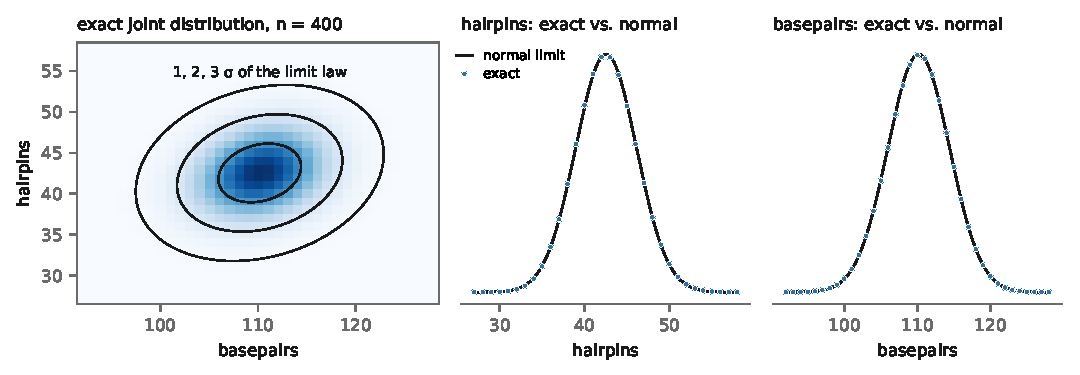
\includegraphics[width=\textwidth]{../figure/joint_distribution.pdf}
\caption{Exact joint distribution of (hairpins, basepairs) at $n=400$ (shading and dots), against the limiting
normal law (ellipses and curves).}\label{fig}
\end{figure}

\section{Formal verification of the algebra}\label{lean}
The file \texttt{lean\_check/LeanCheck/Basic.lean} proves the following in Lean~4 with Mathlib, over an arbitrary field
of characteristic zero or, where $\sqrt5$ is involved, over $\mathbb R$ with a symbol $\mathtt{s}$ standing for $\sqrt5$
and subject only to $\mathtt{s}^2=5$ (and $\mathtt{s}>0$ for the inequalities): the factorization \eqref{fact}; the functional equation of Lemma~\ref{gf} for
$S=1+X+F$, for any $r$ with $r^2=R$; $R(\rho_0,1,1)=0$; the complete Taylor expansion of $R$ at $(\rho_0,1,1)$, which
certifies all partial derivatives of $R$ there, in particular $\partial_XR=30-14\sqrt5\ne0$; the first- and
second-order implicit-differentiation identities satisfied by the Taylor coefficients of $\rho(e^s,e^t)$; the values of
$\mu$ and $H$ obtained from them; $\det H=(13\sqrt5-29)/50>0$, $H_{11}>0$, $H_{12}>0$,
$H_{12}^2=\tfrac{5\sqrt5-11}{4}H_{11}H_{22}$; and $Q(\rho_0)=36\sqrt5-80>0$. All twenty-one theorems are accepted by the
kernel with no axioms beyond the three standard ones (\texttt{propext}, \texttt{Classical.choice},
\texttt{Quot.sound}). Mathematica is used only to propose the polynomials; Lean re-verifies them from scratch.

\emph{Not} formalized: the analytic part of the argument (Lemma~\ref{local}, Lemma~\ref{coef}, L\'evy's theorem) and
the elementary calculus that connects the identities above to the derivatives of $U=-\log\rho$. The value of
$\nabla W(0)$ is machine-verified in Mathematica only.

\subsection*{Code} All scripts, their outputs and the Lean project are at
\url{https://github.com/bshepp/rna-joint-normality}.

\begin{thebibliography}{99}
\bibitem{BR} E. A. Bender and L. B. Richmond, \emph{Central and local limit theorems applied to asymptotic enumeration
II: multivariate generating functions}, J. Combin. Theory Ser. A \textbf{34} (1983), 255--265.
\bibitem{B} AJ Bu, \emph{A Maple package for computing generating functions enumerating RNA secondary structures},
\url{https://sites.math.rutgers.edu/~zeilberg/tokhniot/RNA.txt}.
\bibitem{BKZ} AJ Bu, M. Kauers and D. Zeilberger, \emph{Statistical analysis of hairpins and basepairs in RNA
secondary structures}, arXiv:2602.19255 (2026); J. Syst. Sci. Complex., to appear;
\url{https://sites.math.rutgers.edu/~zeilberg/mamarim/mamarimhtml/rna.html}.
\bibitem{CM} J. A. Cuesta and S. Manrubia, \emph{Enumerating secondary structures and structural moieties for circular
RNAs}, J. Theor. Biol. \textbf{419} (2017), 375--382; arXiv:1607.04435.
\bibitem{D} M. Drmota, \emph{Random Trees}, Springer, 2009.
\bibitem{FS} P. Flajolet and R. Sedgewick, \emph{Analytic Combinatorics}, Cambridge Univ. Press, 2009.
\bibitem{GR} Z. Gao and L. B. Richmond, \emph{Central and local limit theorems applied to asymptotic enumeration IV:
multivariate generating functions}, J. Comput. Appl. Math. \textbf{41} (1992), 177--186.
\bibitem{HK} C. Heuberger and S. Kropf, \emph{Higher dimensional quasi-power theorem and Berry--Esseen inequality},
Monatsh. Math. \textbf{187} (2018), 293--314.
\bibitem{H} H.-K. Hwang, \emph{On convergence rates in the central limit theorems for combinatorial structures},
European J. Combin. \textbf{19} (1998), 329--343.
\bibitem{JSZ} C. Jardon, B. Sheppard and V. Zaveri, \emph{A motion planning algorithm in a figure eight track},
PUMP J. Undergrad. Res. \textbf{6} (2023), 224--249; arXiv:2403.05570.
\bibitem{JR} E. Y. Jin and C. M. Reidys, \emph{Central and local limit theorems for RNA structures}, J. Theor. Biol.
\textbf{250} (2008), 547--559; arXiv:0707.4281.
\bibitem{P} J. S. Padhi, \emph{Solutions to five challenge problems in enumerative and algorithmic combinatorics, with
an account of the human--machine methodology employed}, arXiv:2608.11290 (2026).
\bibitem{PH} S. Poznanovi\'c and C. E. Heitsch, \emph{Asymptotic distribution of motifs in a stochastic context-free
grammar model of RNA folding}, J. Math. Biol. \textbf{69} (2014), 1743--1772; arXiv:1204.3670.
\end{thebibliography}
\end{document}
